\documentclass{exam}

\usepackage{ctex}
\usepackage{amsmath}
\usepackage{physics}
\usepackage{anyfontsize}
\usepackage{esvect}
\usepackage{tikz}

\renewcommand{\thequestion}{\zhnum{question}}
\renewcommand{\questionlabel}{\thequestion .}
\renewcommand{\thepartno}{\arabic{partno}}
\renewcommand{\partlabel}{\thepartno .}
\author{复卷人:王飞扬}
\title{2023春季学期电动力学期中考试(王漱明)}

\begin{document}
\maketitle
\noindent
{\LARGE {\heiti 简答题}}
\begin{questions}
    \question 运用静电唯一性定理解释接地导体球壳内、外的静电屏蔽现象
    \question 分别写出真空中和介质中电磁场的能量密度和能流密度的表达式
    \question 阐述磁矢势 $\vv{A}$ 的物理意义. 列举一个关于$\vv{A}$ 的可观测物理效应,并简述
    \question 写出格林函数$G$ 的物理意义及其满足的微分方程,并分别写出满足两类边值问题的格林函数的边界条件表达式
    \question $\vv{m}$ 是常矢量,$\vv{R}$ 是场点相对原点的位矢,
    定义${ \vv{A}=\frac{\vv{m}\times\vv{R}}{R^3}}$ , ${ \varphi=\frac{\vv{m}\cdot\vv{R}}{R^3}}$,
    试证明$\vv{A}$ 的旋度等于$\varphi$ 的负梯度,即$\nabla\times\vv{A}=-\nabla\varphi$
\end{questions}
\noindent
{\LARGE {\heiti 计算题}}
\begin{questions}
    \question 如图所示,三个带电量分别为$-q,+2q,-q$ 的点电荷在同一直线上排列,两电荷间距为$a$。由此形成线性电四极子体系. 试求在$R>>a$ 处该线性电四极子产生的电势$\varphi^{(2)}$
    \tikzset{every picture/.style={line width=0.75pt}} %set default line width to 0.75pt        
    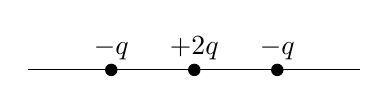
\begin{tikzpicture}[x=0.75pt,y=0.75pt,yscale=1,xscale=1]
        %uncomment if require: \path (0,300); %set diagram left start at 0, and has height of 300

        %Shape: Boxed Line [id:dp7682528906653234] 
        \draw    (0,0) -- (160,0) ;
        \fill (40,0) circle (3);
        \node at (40,0) [above] {$-q$};
        \fill (80,0) circle (3);
        \node at (80,0) [above] {$+2q$};
        \fill (120,0) circle (3);
        \node at (120,0) [above] {$-q$};
    \end{tikzpicture}
    %\label{线性电四极子}
    %\caption{线性电四极子}
    \question 如图所示,一半径为$R$ 的导体球,左右距球心$d$ 处各有一带电量为$q$ 的点电荷
    \begin{parts}
        \part 导体球接地,试证明点电荷不受力的条件与带电量$q$ 的大小无关,只与导体球的半径$R$ 有关; 并写出点电荷不受力时$R=R_0$ 满足的方程
        \part 导体球半径为$R_0$,但不接地,其电势为$\varphi_0$ .求导体球表面总带电量$Q$ 和每个点电荷所受到的力
    \end{parts}
    \begin{tikzpicture}[x=0.75pt,y=0.75pt,yscale=1,xscale=1]
        \draw (100,0) circle (100);
        \fill (100,0) circle (3);
        \node at (100,0) [above] {\large $O$};
        \fill (-60,0) circle (3);
        \node at (-60,0) [above] {\large$q$};
        \draw (-100,0)--(300,0);
        \fill (260,0) circle (3);
        \node at (260,0) [above] {\large$q$};
        \draw [ |<->| ] (-60,-7)--node[below]{\large $d$}(100,-7);
    \end{tikzpicture}
    \question 一半径为$R$ 的导体球壳置于电场强度为$\vv{E_0}$ 的均匀场中
    \begin{parts}
        \part 球壳电势为$\varphi_S$ ,用Laplace方法求解球壳外的电场分布和球壳上的电荷分布
        \part 若球壳不带电,沿与$\vv{E_0}$ 垂直的方向将球壳分割为2个半球壳,求需要施加多大的外力使得两个半球壳不被分开
    \end{parts}
    \question 对于电流密度为$\vv{J}(\vv{R'})$ 的电流体系,其磁矢势的表达式为$\vv{A}(\vv{R})={\displaystyle\frac{\mu_0}{4\pi}\int_{V'}\frac{\vv{J}(R')}{r}\dd V'}$ .磁矢势可以写成多极展开的形式,即$\vv{A}=\vv{A}^{(0)}+\vv{A}^{(1)}+\vv{A}^{(2)}+ \cdots$
    \begin{parts}
        \part 写出磁多极展开的具体表达式
        \part 证明$\vv{A}^{(0)}=0$ ,并解释其物理意义
        \part 证明${\displaystyle \vv{A}^{(1)}=\frac{\mu_0}{4\pi R^3}\vv{m}\times\vv{R}}$
    \end{parts}
    \question 在磁场强度为$\vv{H_0}$ 的均匀外场中,有一半径为$R_0$ 的均匀介质球,磁导率为$\mu$.求:
    \begin{parts}
        \part 球内外的磁感应强度$\vv{B}$.
        \part 产生的诱导磁矩$\vv{m}$
        \part 球内的磁化电流密度$\vv{J_M}$和球表面的磁化电流面密度$\vv{\alpha_M}$
    \end{parts}
\end{questions}
\end{document}